\typeout{NT FILE preliminary-work.tex}

\prependtographicspath{{Chapters/Figures/}}

\glsresetall

\chapter{Preliminary Work}
\label{cha:preliminary_work}

As stated in Chapter~\ref{cha:introduction}, the adoption of \gls{MAS}s as \gls{CPPS}s for Industry 4.0 has not been as widespread as desired. It never left the prototyping stage and therefore never evolved in an industrial environment and never improved in a practical setting. This work seeks to alleviate some of this by suggesting a method to more easily create new Industrial Agents, capable of interfacing with industrial hardware.

\section{Base Framework}
\label{sec:base_framework}

In this work we propose a marketplace framework capable of integrating any kind of device, from high level computational interfaces to simple \gls{PLC}s for hardware interfacing. This system should be capable of easily integrating new hardware by picking from a set of generic libraries. A developer wanting to add new hardware to the system should be able to specify what kind of device it is, and then the proposed framework picks from a database the most adequate libraries for that specific device. The developer should be able to then tweak these configurations to better suit the expected behaviors the new hardware should follow in the production line. An example of the systems architecture can be found in Figure~\ref{fig:example_architecture}. As an alternative, this system may also be capable of integrating any kind of hardware with any kind of agent, through the use of these generic libraries, an example is shown in Figure~\ref{fig:bonus_architecture}.\\

\begin{figure}[h!]
	\centering
	\subbottom[Example Architecture\label{fig:example_architecture}]{%
		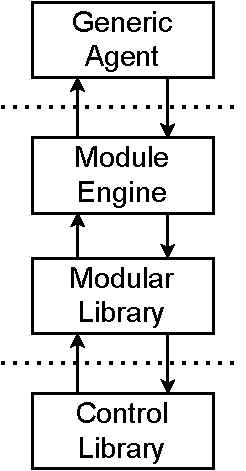
\includegraphics{ExampleArchitecture}}%
	\subbottom[Alternative Architecture\label{fig:bonus_architecture}]{%
		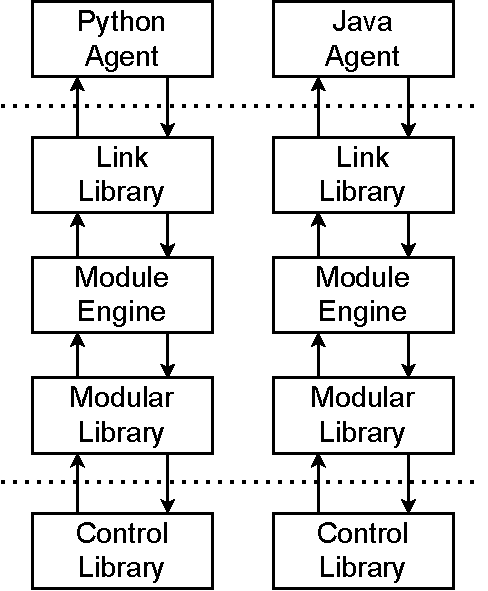
\includegraphics{BonusArchitecture}}%
	\caption{System Architectures}
	\label{fig:system_architectures}
\end{figure}

In both Figure~\ref{fig:example_architecture} and Figure~\ref{fig:bonus_architecture}, the Module Library is the part of the system that selects the correct libraries to use. It then implements them as a Modular Library, that then interfaces with the hardware. Since this systems work from a high layer to a lower layer, it could also work in the opposite direction. The Module Engine could also pick libraries to interface with the agent above and implement them as a Link Library. This would allow the system to integrate any kind of agent with any kind of hardware.\\\\\\

The project development plan follows this order, and in Table~\ref{tab:timeline} the development timeline is shown:
\begin{enumerate}
	\item Design the system architecture
	\item Implement the platform
	\item Implement the test libraries
	\item Validation and testing
	\item Writing the dissertation
\end{enumerate}

\begin{table}[h!]
	\centering
	\caption{Project timeline}
	\begin{tabular}{||l||c|c|c|c|c|c|c|c||}
		\toprule
		\hline
		{} 				         & February 		 & March 			 & April             & May               & June              & July              & August            & September\\
		\hline
		Design architecture 	 & \cellcolor{green} & \cellcolor{green} & 		             &                   &                   &                   &                   & \\
		\hline
		Implement platform 		 & 					 & \cellcolor{green} & \cellcolor{green} & \cellcolor{green} &                   &                   &                   & \\
		\hline
		Implement test Libraries & 					 &                   &                   & \cellcolor{green} & \cellcolor{green} &                   &                   & \\
		\hline
		Testing and validation 	 & 					 &                   &                   &                   & \cellcolor{green} & \cellcolor{green} &                   &  \\
		\hline
		Writing Dissertation     & 					 &                   &                   &                   &                   & \cellcolor{green} & \cellcolor{green} & \cellcolor{green} \\
		\hline
		\bottomrule
	\end{tabular}
	\label{tab:timeline}
\end{table}

\subsection{Design}

During the design stage of the project, the main features and requirements will be delineated. The base system architecture will be designed and the main programming language with which the system will be made will be chosen.

\subsection{Implementation}

At the implementation stage, the platform will be developed. Its main features will be implemented, such as the way users will configure the libraries. The system architecture may still be adapted at this point to better fit the requirements.

\subsection{Test Libraries}

During this stage, test libraries for the platform will be developed. These test libraries would simulate the database that the platform is dependent on to create the modules for the new industrial agents that will be integrated into the simulated \gls{CPPS}. 

\subsection{Validation and Testing}

Finally, the system will be evaluated with multiple tests to check the robustness and flexibility of the system

\subsection{Writing the dissertation}

This stage is self-explanatory, the dissertation will be written to record the whole process of development, implementation and testing.\\